%=================================================================
\documentclass[dvipdfmx]{issj}
%=================================================================
% 情報システム学会 研究発表大会 原稿用テンプレートの利用例
%     ISSJ実行委員会/プログラム委員会(ISSJ学会誌編集委員会)
% issj2012.sty Ver. 0.50 2012-10-12 Tadashi Iijima (iijima@ae.keio.ac.jp)
% issj2012.sty Ver. 0.60 2012-10-15 Tadashi Iijima (iijima@ae.keio.ac.jp)
% issj2012.sty Ver. 0.70 2012-10-19 Tadashi Iijima (iijima@ae.keio.ac.jp)
% issj2012.sty Ver. 0.80 2012-10-20 Tadashi Iijima (iijima@ae.keio.ac.jp)
%=================================================================
\title{「Twitter上で共感を生み出すツイートの性質に関する考察」の検証}
%-----------------------------------------------------------------
\etitle{Verification of "Consideration on Characteristics of Sympathy-arousing Tweets on Twitter"}
%-----------------------------------------------------------------
\author{木村 咲\uddag, 松澤芳昭\uddag}
%-----------------------------------------------------------------
\eauthor{Saki Kimura\udag, and Yoshiki Matsuzawa\uddag}
%-----------------------------------------------------------------
\affiliation{\dag 青山学院大学 社会情報情報学部\ddag }
%-----------------------------------------------------------------
\eaffiliation{\dag School of Social Informatics, Aoyama Gakuin University.}
%-----------------------------------------------------------------
%=================================================================
\begin{document}
%=================================================================
\maketitle
%=================================================================
\begin{abstract}
本研究では、先行研究で実証されていた「Twitter上で共感を生み出すツイートの性質」の再現性を確認することを目的に分析を行う。 本稿では先行研究とは異なるツイートデータを対象とし、新たに属性として「画像の有無」と「感情極性値」を追加した。 芸能人4名のデータを収集して分析した結果、全ての属性においてTwitterで共感を生み出す性質は見られなかった。 これは先行研究と(A)ツイートの時期、(B)ラベル付けした被験者が異なるためだと考えられる。
\end{abstract}






%=================================================================
%=================================================================
%=================================================================
%=================================================================
%=================================================================
\section{はじめに} %%%% 第1節
%=================================================================

近年はSNS上で買い物ができたり、YoutuberやインスタグラマーなどSNSを使った職業も増え、今後よりSNSマーケティングは盛んになると考えられる。
中でもSNSを運用するにあたって共感の注目が高まっており、日本企業の約63.9%が「SNS運用でユーザーの共感の獲得が目標の指標になっている」と答えている[1]

Twitterでの共感の研究[2]では、不特定の相手向けにされたツイートに共感を抱くケースに着目し、その発生のメカニズムの解明を目的としTwitter上で共感を生み出すツイートの性質について研究している。
その結果、「文字数が少ないツイート」と「悲しみを含むツイート」が共感を生み出しやすいことが判明した。文字数が関与してる理由としては、ツイートが長いほどユーザーがテキスト全てを読まなくなり、共感発生の妨げになっている可能性があるからだ。
また、悲しみを含むツイートの方が共感を発生しやすくなる理由は、悲しい記憶は人間の心に残りやすく、そのためツイートを投稿したユーザーの状況をイメージしやすくなり、共感を発生する可能性が高くなるためだと考察している。

そこで本稿では、先行研究の結果は再現可能なのかの検証を行う。
加えて、画像付きのツイートの方がユーザーはツイートの内容をイメージしやすくなり、共感発生の手助けになると考え、新たな属性として「画像有無」も加え実験を進める。




%=================================================================
%=================================================================
%=================================================================
%=================================================================
%========================================================================
\section{共感の定義}  %%%% 第2節
%========================================================================
本稿では先行研究とは異なる共感の定義づけを行う。
先行研究ではTwitterにおける共感を「そのツイートを不特定多数のユーザーが閲覧したときに,投稿した背景が想像でき,それに同感できる」ことと定義している。
この定義の場合、ツイートに同感できなければ共感は成り立たないことを意味している。


しかし、佐伯は「同感」と「共感」を別物と捉えている。
佐伯曰く、「同感というのはその人の感じていることと自分の感じていることを同じなのだと思うこと」。
一方の共感は、「白分にはすてきとは思えないが,その良さをわかりたい」などというように、探求して「理解」しようとすることと捉えられている。[3]
ロジャーズは共感を「自分が自分が他者であるかのような、しかし”かのようにas if”という状態を失わずに関係する。正確さや感情的要素、意味を持って他者の内部関連気分を知覚すること」と唱えている。[4] 
本稿では、この2つをもとに共感を、「不特定多数のユーザーがそのツイートを閲覧したとき、投稿した背景が想像でき、そのツイート(投稿者)の内部関連気分を汲み取れること」と定義する。



%========================================================================
\section{研究方法}  %%%% 第3節
%========================================================================
本稿では先行研究とは異なる方法で実験を進めている。
先行研究との違いについて表1に示す。



%%%% 表:先行研究との比較
\begin{table}
  \caption{先行研究との比較}
\begin{tabular}{c|c|c} \hline\hline
  & 先行研究 & 本研究 \\\hline
%%%% ① 共感の定義
 共感の定義  &
  \begin{tabular}{l}
{\small   \begin{tabular}{l}
投稿した背景が想像でき、\\
その投稿に同感できること
  \end{tabular}}   

  \end{tabular} &

{\small   \begin{tabular}{l}
投稿した背景が想像でき、\\
投稿者の内部関連気分を汲み取れること
  \end{tabular}}   
 \\\hline

%%%%② ツイート対象

ツイート対象  & {\small 芸能人5名} &  {\small 芸能人4名} \\\hline


%%%%③ ラベル付け

ラベル付け  &  {\small 第一著者による手作業} & {\small 第一著者による手作業}  \\\hline

%%%% ④ 分析方法
分析方法  &  {\small 機械学習} & {\small 手作業}  \\\hline

%%%% ④ 属性
属性 &
 {\small   \begin{tabular}{l}
    いいね数\\
    リツイート数\\
    文字数\\
    時間間隔\\
    非公式リツイート\\
    喜怒哀楽\\
    肯定的 or 否定的 or 中立\\
    賛成的 or 反対的 or 中立\\
  \end{tabular}}
 &
 {\small   \begin{tabular}{l}
    文字数\\
    画像有無\\
    感情極性値\\
  \end{tabular}}
 \\\hline



 \end{tabular}
\end{table}




%------------------------------------------------------------------------
\subsection{ツイートの収集方法 }  %%%% 第3.1節
%------------------------------------------------------------------------
今回は芸能人の中でもフォロワー数が最も多い芸能人男女4名を分析対象とし、2021年7月27日から最新のツイートをそれぞれ50件ずつ収集した。
第一次情報源でない「公式リツイート」と、特定の相手に対してのつぶやきである「リプライ」は除いている。




%------------------------------------------------------------------------
\subsection{共感のラベル付け  }  %%%% 第3.2節
%------------------------------------------------------------------------
共感のラベル付けは、表2の2つの条件が成り立つときに行う。



ラベル付けの例を表3に示す。
左は「共感を生み出す」とラベル付けされたツイートである。
このツイートからは、投稿者が”自分の誕生日に周りに祝ってもらって嬉しくてツイートした”という背景(条件1)と、”祝ってもらって嬉しい”という感情(条件2)が読み取れる。
一方で、右は「共感を生み出さない」とラベル付けされたツイートである。
このツイートからは、吉高由里子が”手持ち花火をしている”というツイートの背景が確認できる(条件1)。
しかし、感情面については言及されていないため、感情を汲み取ることはできない。
つまり、条件2を満たしていないため、共感を生み出さないツイートとラベル付けした。

%%%% 表2:ラベル付けの判断基準
\begin{table}[t]\centering
\caption{ラベル付けの判断基準}\label{tbl:font}
\begin{small}
\begin{tabular}{c|c} \hline\hline
No & 条件内容\\\hline
条件1& ツイートの背景が想像できるツイート\\
条件2 & 投稿者の感情が汲み取れるツイート\\\hline
\end{tabular}
\end{small}
\end{table}


%%%% 表3:共感を生み出すツイートの例
\begin{table}[t]\centering
  \caption{共感を生み出すツイートの例}
  \begin{tabular}{c|c} % l:左寄せ,c:中央揃え r:右寄せ 
\hline\hline \rm 共感を生み出すツイート & \rm 共感を生み出さないツイート \\ \hline 
    \begin{minipage}{70mm}
      \centering
      \scalebox{0.3}{
\includegraphics{fig1.png}}
    \end{minipage} &
    \begin{minipage}{70mm}
      \centering
      \scalebox{0.3}{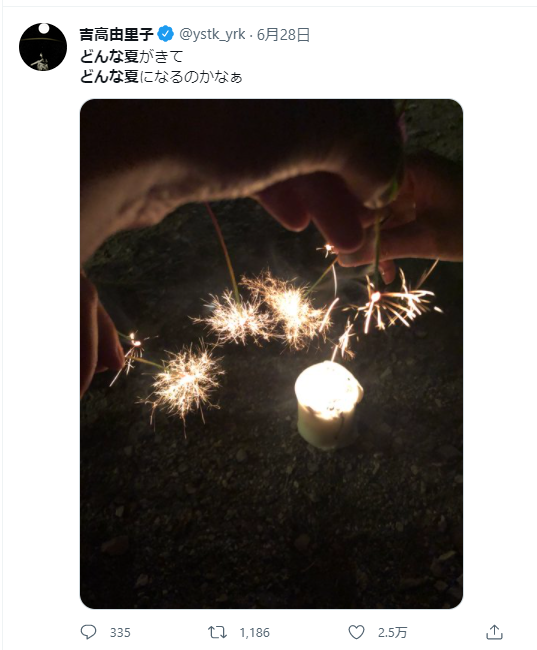
\includegraphics{fig2.png}}
    \end{minipage} \\ \hline
  \end{tabular}
  \label{pic} % \ref{ラベル名}で表番号を参照
\end{table}



%------------------------------------------------------------------------
\subsection{属性の定義と抽出方法}  %%%% 第3.2節
%------------------------------------------------------------------------
ここでは本稿で用いる属性について説明する。
先行研究で共感の発生と関係があるとされていた「文字数」と「悲しみの感情」は本当に共感発生に影響を及ぼしているのか、そして「画像の有無」も共感発生の手助けになってるのではないかを検証するため、表4の3つの属性「文字数」「画像有無」「感情極性値」を用いる。以下にそれぞれの属性について説明していく。


\subsubsection{【文字数】}
1つ目の文字数は対象ツイートの文字数を指している。先行研究ではツイートの長さが長いほど共感の発生を妨げになっていると考えられていた。[3]

\subsubsection{【画像有無】}
2つ目の画像有無はツイートに画像が添付されているか否かを表している。画像の有無は読み手にツイート内容をイメージしやすくさせる役割を果たし、共感発生にも影響を及ぼしているという仮説があり、新たに属性として加えた。

\subsubsection{【感情極性値】}
最後に感情極性値はツイートテキストのネガティブ(ポジティブ)評価ができる感情極性値のことを指している。先行研究では感情語辞書を作成し、ツイートテキストに喜怒哀が含まれているかどうかを分析を行っていたが、本稿では感情極性値を用いる。[5]この値は最小に近くなるほど、そのツイートはネガティブと判断できる。

%%%% 表:属性名と属性値の形式
\begin{table}[t]\centering
\caption{属性名と属性値の形式}\label{tbl:font}
\begin{small}
\begin{tabular}{c|c} \hline\hline
属性名            & 属性値の形式\\\hline
文字数         & real 型, 0~\\
画像有無 & {yes, no}\\
感情極性値     &  real 型, -1~1\\\hline
\end{tabular}
\end{small}
\end{table}

%------------------------------------------------------------------------
\subsection{性能評価の方法}  %%%% 第3.2節
%------------------------------------------------------------------------
表4に示した各ツイートの属性値を「説明属性」、共感発生の有無を「目的属性」と定めてデータセットを作成し、適合率、再現率により性能を評価する。(表5)


%%%% 表:データセットの概要
\begin{table}[t]
  \caption{データセットの概要}
  \label{table:data_type}
  \centering
  \begin{tabular}{c|c|r}
    \hline\hline
   ユーザー名 & フォロワー数  &  共感発生数  \\
    \hline 
吉高由里子 & 310.0万人 &  22/50  \\
ベッキー & 195.1万人 &  25/50  \\
松本人志 & 818.9万人 &  20/50  \\
有吉弘行 & 671万人 &  6/50 \\
    \hline
  \end{tabular}
\end{table}





%========================================================================
\section{結果と考察}  %%%% 第4節
%========================================================================
結果を表5に示す。以下にそれぞれの考察を述べる。


%%%% 表:結果
\begin{table}[t]
\centering
  \caption{結果}
  \begin{tabular}{c|c|c|c|c|c|c}  \hline\hline
 &  \multicolumn{2}{|c|}{文字数} &  \multicolumn{2}{|c|}{画像有無} &  \multicolumn{2}{|c|}{感情極性値} \\ \hline
&適合率 & 再現率 & 適合率 & 再現率 &適合率 & 再現率 \\\hline
吉高由里子 & 0.2&0.09 &0.38&0.27 & 0.41&0.41 \\
ベッキー& 0.11&0.16 &0.5&0.08& 0.46&0.44 \\
松本人志& 0.32&0.45 & 0.67&0.1 &0.31&0.45\\
有吉弘行& 0.09&0.67 & 0.08&0.33 &  0.11&0.33 \\ \hline

  \end{tabular}
\end{table}


%------------------------------------------------------------------------
\subsection{【文字数の考察】}  %%%% 第4.2節
%------------------------------------------------------------------------
1つ目の文字数は、先行研究の結果とは異なり、文字数が少ないと共感が発生する傾向は確認できなかった。
先行研究では、文字数がある値以下のときに共感を生み出すという学習結果が多く見られ、文字数が多いとユーザーがテキスト全てを読まなくなり共感発生の妨げになっているのではないか、短く要点がまとまってる文章の方が共感を発生させやすいのではないかと考察していた。

しかし、今回のデータからは文字数の少なさと共感発生に関係は見られなかった。
認知的共感に基づいて考えると、共感するにはまず相手の状況をしっかり理解する必要がある。
そのため、ツイート内容に投稿者の考えやできごとの詳細が記載が少ない文字数の少ないツイートは共感は発生しにくいのかもしれない。

%------------------------------------------------------------------------
\subsection{【画像有無の考察】}  %%%% 第4.2節
%------------------------------------------------------------------------
2つ目の画像の有無は、投稿した背景や投稿内容がイメージしやすく共感が発生しやすいと予想していたが、これも同様に共感発生との関係は見られなかった。

画像を用いることでツイートの背景や内容を理解しやすくなるという側面はあるが、その画像の内容も考慮する必要がある。
今後はツイート内容と画像の内容がマッチしているのか、なども踏まえたうえで分析する必要がある。

%------------------------------------------------------------------------
\subsection{【感情極性値の考察】}  %%%% 第4.2節
%------------------------------------------------------------------------
最後に感情極性値も共感発生との関係は見られなかった。
今回使用した単語感情極性値での分析方法では、そのツイートが意味する感情を正確に測れていない可能性があるため、人の手によって判定する必要があることも検討しなければいけない。

%------------------------------------------------------------------------
%------------------------------------------------------------------------
%------------------------------------------------------------------------





%------------------------------------------------------------------------
%------------------------------------------------------------------------
%------------------------------------------------------------------------%------------------------------------------------------------------------
%------------------------------------------------------------------------
%------------------------------------------------------------------------




%------------------------------------------------------------------------
%------------------------------------------------------------------------
%------------------------------------------------------------------------%------------------------------------------------------------------------
%------------------------------------------------------------------------
%------------------------------------------------------------------------



%========================================================================
\section{おわりに}  %%%% 第5節
%========================================================================

本稿では、先行研究に基づいてTwitterにおいて共感を発生させるツイートにはどのような性質があるのかを調査し考察を行った。

分析結果より、先行研究でいわれていた文字数が少ないツイートが共感を発生させることは検証できなかった。
また、ツイートのポジティブ(ネガティブ)さを表す感情極性値や画像の有無からも共感発生の関係は見ることができなかった。





%========================================================================
%%%% 参考文献
%========================================================================
\begin{thebibliography}{99}


  \bibitem{bib:SO2014} 坂田利康, 
                       ^^ ^^ SNSマーケティング戦略 Facebookを使った価値共創による商品開発、総合的O2O、ユーザー・アナリティクスの事例による一考察 '' 
                       高千穂論叢 ,Vol.49 No.3, 2014, pp.83-142.

  \bibitem{bib:HV1987}  大川 陽聡,高間 康史, 
                       ^^ ^^ Twitter 上で共感を生み出すツイートの性質に関する考察 '' 
                       インタラクティブ 情報アクセスと可視化マイニング研究会 ,Vol.2012 NoAM-02,2012, pp.02-.



  \bibitem{bib:NT2017} 佐伯 胖,
                       ^^ ^^ 「子どもがケアする世界」をケアする:保育における「二人称的アプローチ」入門'' 
                       ミネルヴァ書房 ,2017.

  \bibitem{bib:NT2010} 福田正治,
                       ^^ ^^ 共感心と心をつなぐ感情コミュニケーション'' 
                       へるす出版 ,2010.
  

  \bibitem{bib:NT2006} 高村大也, 乾考司, 奥村学,
                       ^^ ^^ “スピンモデルによる単語の感情極性抽出,” 情報処理学会論文誌 Vol.47 No.2, pp.627-637,2006.





\end{thebibliography}
%========================================================================
\end{document}
%========================================================================
